\section{K7 -- Generowanie realistycznych obrazów scen 3-D za pomocą metody śledzenia promieni}

\textbf{Fotorealizm} jest to metodyka starająca się w jak najlepszym stopniu oddać świat rzeczywisty za pomocą wygenerowanego obrazu. Aby to osiągnąć wykorzystuje się różne metody takie jak \textit{fotogrametria} (łączenie zdjęć tego samego obiektu z wielu różnych perspektyw w celu wygenerowania obiektu 3-D - technologia użyta np. przy tworzeniu gry \textit{The Vanishing of Ethan Carter}), metody próbkowania przestrzeni, czy też metoda śledzenia promieni. 

\textbf{Metoda próbkowania przestrzeni} polega na analizowaniu toru promieni od źródła światła, poprzez odbicia od obiektów sceny, aby finalne trafić do oka obserwatora albo wylecieć poza scenę. Z każdego źródła światła wyprowadzany jest pęk promieni (\textbf{dyskretyzacja światła}), i im więcej promieni, tym dokładniejszy stanie się obraz. Tutaj pojawia się problem, gdyż generowana jest bardzo duża liczba promieni, z czego ogromna większość nie przecina nawet rzutni (nie dociera do oka obserwatora), przez co operacje wykonane zostały bezsensownie. Stąd też wymyślona została metoda śledzenia promieni rozwiązująca ten problem.

\textbf{Metoda śledzenia promieni} (ang. \textit{Ray Tracing}) jest techniką służącą do generowania fotorealistycznych scen trójwymiarowych 3-D. Opiera się na śledzeniu wyłącznie tych promieni, które docierają do obserwatora. Cechą charakterystyczną jest to, że promienie nie są analizowane normalnym torem, tj. od źródła światła, bądź światła odbitego, do obserwatora, lecz właśnie \textbf{od oka obserwatora do elementów na scenie}. Zatem dla każdego piksela obrazu wynikowego wyprowadzany jest jeden promień, od którego w następstwie zależy wartość koloru tego piksela.

Wyprowadzony promień może nie trafić w żaden obiekt na scenie - piksel przyjmuje wtedy określony kolor tła. Promień może także trafić na źródło światła - piksel zyskuje kolor źródłowy światła. Promień może również trafić w jakiś obiekt na scenie. Jeśli trafi na taki obiekt, to wyznaczane są \textbf{punkty przecięcia}, następnie brany jest punkt przecięcia najbliższy początkowi promienia (gdyż punktów przecięcia dla obiektu może być kilka) i dla niego obliczany jest kolor punktu za pomocą wybranego modelu oświetlenia, na przykład popularnego \textbf{modelu Phonga}. Obliczane są w tym momencie także cienie używając pomocniczych promieni biegnących do źródła światła - gdy wiązka przetnie inny obiekt to oryginalny punkt jest zaciemniony. Całą procedurę można następnie powtarzać rekurencyjnie śledząc kolejne promienie odbite (zwane wtórnymi) i załamane tak, aby uzyskać efekt przedmiotów odbijających się w sobie nawzajem.

Przebieg działania algorytmu zapisywany jest w postaci \textbf{drzewa} (graf nieskierowany). Skrócony przebieg algorytmu przedstawić można w kilku krokach:
\begin{enumerate}
	\item Dla każdego piksela obrazu wyprowadź \textbf{promień pierwotny}.
    \item Dla każedgo napotkanego obiektu oblicz odbicia i wyprowadź \textbf{promienie wtóre}. Każdy punkt odbicia zapisz jako nowy węzeł drzewa.
    \item Dla każdego węzła wyznacz oświetlenie lokalne korzystając z wybranego modelu oświetlenia.
    \item Przechodząc od liści drzewa dodawaj kolejne wartości oświetlenia lokalnego ustalając tym samym ostateczną wartość piksela, od którego wyszedł promień pierwotny.
\end{enumerate}

Algorytm kończy swe działanie w momencie, gdy:
\begin{itemize}
	\item Promień nie trafia w żaden obiekt na scenie
    \item Promień trafia w obiekt całkowicie rozpraszający światło
    \item Promień trafia na obiekt, w którym następuje całkowite wewnętrzne odbicie
    \item Wyczerpana została ilość rekursywnych odbić
\end{itemize}

\textbf{Model Phonga} służy do wyznaczania oświetleń lokalnych. Na model ten składają się trzy rodzaje oświetlenia:
\begin{enumerate}
	\item \textbf{Światło ambientowe} - światło otoczenia, jest to wartość stała przypisana do danej sceny.
	\item \textbf{Światło rozproszone} - podstawowy kolor obiektu, wyliczany na podstawie \textbf{modelu Lamberta} (\textit{Lambert, Lambert ty chuju} - Wiedźmin Geralt z Rivii) i widoczny przede wszystkim na powierzchniach matowych (drewno, papier).
	\item \textbf{Światło odbite} - odpowiada za efekt połysku dla powierzchni śliskich, błyszczących (Passat metallic nówka nie śmigana trzy razy klepana). Wskazuje kierunek promienia odbitego.
\end{enumerate}

\begin{figure}[!h]
\centering
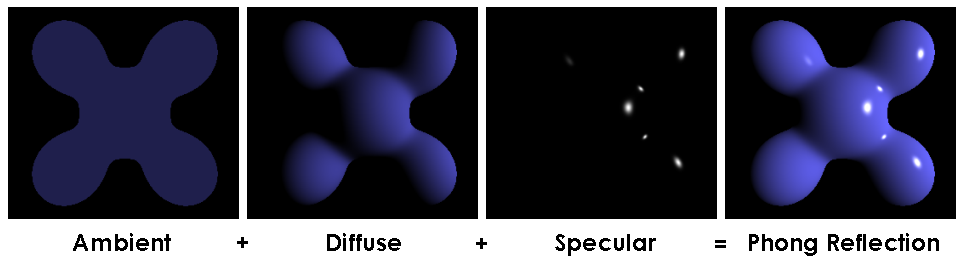
\includegraphics[width=0.8\textwidth]{k7_model_phonga.png}
\caption{Model Phonga}
\end{figure}

Owe składowe są mnożone przez procentowy współczynnik wpływu każdej składowej a następnie sumowane według poniższego wzoru:

\begin{equation}
I = k_{a}I_{a} + k_{d}I_{d} + k_{s}I_{s}
\end{equation}

Gdzie:
\begin{itemize}
	\item $I$ – natężenie światła w punkcie
	\item $I_{a}$ – (ang. \textit{ambient}) natężenie światła otoczenia
    \item $I_{d}$ – (ang. \textit{diffuse}) natężenie światła rozproszonego
    \item $I_{s}$ – (ang. \textit{specular}) natężenie światła odbitego lustrzanie
	\item $k$ – procentowy współczynnik wpływu składowych (przypisane do danego obiektu)
\end{itemize}

\textbf{Prawo Lamberta} mówi, że natężenie światła rozproszonego jest wprost proporcjonalne do kosinusa kąta pomiędzy wektorem promienia a wektorem normalnym do powierzchni. W skrócie - im mniejszy kąt, tym mniej światła jest rozproszone (powierzchnia skierowana prostopadle do promienia jest najjaśniejsza).

W modelu Phonga używany jest także dodatkowy efekt zway \textbf{tłumieniem atmosferycznym}, polegające na spadku natężenia światła wraz z rosnącą odległością od obserwatora. Zjawisko to można wykorzystać do generacji realistycznych warunków pogodowych, takich jak deszcz, zamieć, mgła.

Metoda śledzenia promieni mimo, że daje zdumiewające rezultaty to ma w sobie kilka poważnych wad:
\begin{itemize}
	\item Jest \textbf{bardzo kosztowna obliczeniowo} przez dużą liczbę obliczeń potrzebnych do wyliczenia koloru każdego piksela. Najbardziej kosztowne jest liczenie kolizji, co optymalizować można np. algorytmem brył otaczających, czyli wpisaniem zaawansowanych brył w większe, prostsze kształty - jeśli nie wystąpi kolizja z prostym kształtem, to na pewno nie nastąpi także z tym zaawansowanym.
    \item Może występować \textbf{zjawisko aliasingu}, które sprawia, że niektóre małe obiekty są pomijane, a obiekty o ostrych krawędziach mogą być zniekształcone (poszarpane). W celu uniknięcia tego problemu stosowanych jest wiele metod \textbf{antyaliasingu} na przykład nadpróbkowanie (\textit{supersampling - SSAA}), gdzie jeden promień pierwotny zastępowany jest \textbf{wiązką promieni} i kolor piksela jest zazwyczaj średnią z tej wiązki
    \item Przyrost ilości źródeł światła i obiektów znacznie pogorsza czas renderowania
    \item Nie wszystkie kierunki padania promieni są rozpatrywane
    \item Każdą klatkę trzeba generować od nowa - nie można wykorzystać informacji z poprzednich klatek
\end{itemize}

Wartym zaznaczenia jest fakt, że \textbf{śledzenie promieni dla każdego z pikseli odbywa się niezależnie} od innych pikseli, także metodę tę można \textbf{zrównoleglić} (zarówno dla grupy pikseli bądź promieni) na przykład wykorzystując zestawy instrukcji MMX oraz SSE z architektury SIMD równoleglące te same operacje arytmetyczne na liczbach całkowitych w procesorze, bądź używając do tego celu dobrodziejstw najnowszych procesorów graficznych - na przykład technologii NVIDIA CUDA, która pozwala na otrzymanie obrazu generowanego tą metodą w czasie rzeczywistym.